% (c) 2015 Daniele Zambelli daniele.zambelli@gmail.com

\chapter{Iperbole}

% \section{TODO}
% 
% \section{Ellisse con centro nell'origine e assi ...}
% \label{sec:01_formacanonica}

% \begin{wrapfloat}{figure}{r}{0pt}
% \includegraphics[scale=0.35]{img/fig000_.png}
% \caption{...}
% \label{fig:...}
% \end{wrapfloat}
% 
% \begin{center} \input{\folder lbr/fig000_.pgf} \end{center}

% \section{Altro paragrafo}
% \label{sec:ellisse_}

\section{L'iperbole}
\label{sec:iperbole_}

\noindent\begin{minipage}{.75\textwidth}
L'iperbole è la conica corrispondente all'intersezione fra un cono a doppia 
falda e un piano più inclinato della retta generatrice. In tal caso infatti il piano 
taglia entrambe le due falde del cono dando origine a una curva illimitata 
costituita da due parti, dette rami.
\end{minipage}
\hspace{.5cm}
\begin{minipage}{.2\textwidth}
  %    \begin{inaccessibleblock}[Cono a due falde tagliato da un piano
  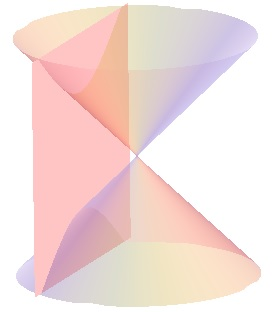
\includegraphics[width=\textwidth]{img/iperbole2.jpg}
  %    \caption{Generazione di un cono a due falde}% 
  %\label{fig:ellissedalcono}
  %    \end{inaccessibleblock}
\end{minipage}  

\subsection{L'iperbole come luogo geometrico}
\label{subsec:iperbole_luogogeometrico}

L'iperbole può essere definita come luogo geometrico, nel seguente modo:
\begin{definizione}
  Dati nel piano $ \pi $ due punti $ F_{1} $ e $ F_{2} $, detti 
fuochi, si dice iperbole il luogo geometrico I dei punti P di $ \pi $ tali 
che sia costante la differenza delle distanze di P da $F_{1}$ e $F_{2}$ 

\begin{equation}
% I=\{P \in\pi|\overline{PF_{1}}-\overline{PF_{2}}=2a,a\in R_{+}^{0}\}
  I=\{P \in\pi \sand \abs{PF_{1}-PF_{2}} = 2a,~2a \geq 0\}
\end{equation}
\end{definizione}

% \begin{figure}[h]
  %\hspace{12pt}
  \begin{minipage}[c]{.70\textwidth}
Leggiamo la formulazione della definizione: la differenza delle distanze 
tra due punti fissati, chiamati \textbf{fuochi}, e un generico punto P dell'iperbole 
risulta fissata e pari a $2a$, qualsiasi sia il punto dell'iperbole. 
Questa lunghezza $(2a)$ è associata ad un numero reale non negativo.
I diversi punti P appartenenti al luogo geometrico dovranno dunque 
mantenere costante la differenza tra le lunghezze dei segmenti 
$\overline{PF_{1}}$ e $\overline{PF_{2}}$ come indicato nella figura a 
fianco:
  \end{minipage}
  \hspace{.5cm}
  \begin{minipage}[c]{.25\textwidth}
    %    \begin{inaccessibleblock}[Cono a due falde tagliato da un piano
    %      che forma un'ellisse.]
    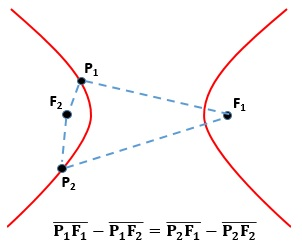
\includegraphics[width=1.1\textwidth]{img/iperbol1.jpg}
%     \caption{L'iperbole come luogo geometrico.}
    %\label{fig:ellissedalcono}
    %    \end{inaccessibleblock}
  \end{minipage}
% \end{figure}

\vspace{7pt}

% \begin{figure}[h]
  %\hspace{12pt}
  \begin{minipage}[c]{.27\textwidth}
    %    \begin{inaccessibleblock}[Cono a due falde tagliato da un piano
    %      che forma un'ellisse.]
    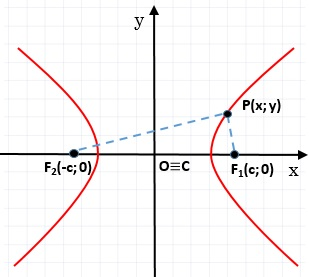
\includegraphics[width=1.1\textwidth]{img/iperbol2.jpg}
%     \caption{i fuochi dell'iperbole.}
    %\label{fig:ellissedalcono}
    %    \end{inaccessibleblock}
  \end{minipage}
  \hspace{.8cm}
  \begin{minipage}[c]{.65\textwidth}
Cerchiamo ora di determinare l'equazione algebrica associata a 
questa curva.
Consideriamo i due fuochi $ F_{1}(-c;~0)$ e $ F_{2}(0;~c)$ sull'asse 
delle X e chiamiamo \textbf{centro} (dell'iperbole) il punto medio del segmento
$\overline{F_{1}F_{2}}$, e \textbf{distanza focale} la misura di tale segmento $\overline{F_{1}F_{2}}$, pari a $2c$.

Applichiamo quindi la definizione $\left|\overline{PF_{1}}-\overline{PF_{2}}\right|=2a$. 

Utilizzando la formula per la lunghezza di un segmento 
possiamo riscrivere la precedente relazione come:
    \(\left|\sqrt{(x-c)^{2}+y^{2}} -\sqrt{(x+c)^{2}+y^{2}}\right|=2a\).
  \end{minipage}
% \end{figure}

Sviluppando i calcoli come si è fatto per l'ellisse, con alcuni passaggi 
algebrici si ottiene l'espressione: $\left( c^{2} -a^{2}\right) x^{2}+a^{2}y^{2}=a^{2}\left(c^{2}-a^{2}\right)$

Applicando la sostituzione $ c^{2}-a^{2}=b^{2} $ 
otteniamo quindi l'equazione: $b^{2}x^{2}-a^{2}y^{2}=a^{2}b^{2}$.  
Dividendo infine entrambi i membri per $a^{2}b^{2}$, si ricava l'espressione:
\begin{equation}
\dfrac{x^{2}}{a^{2}}-\dfrac{y^{2}}{b^{2}}=1
\end{equation}
detta equazione canonica dell'iperbole avente i fuochi sull'asse X.

\subsection{Le caratteristiche dell'iperbole}
\label{subsec:iperbole_caratteristiche}

\begin{description}
\item [\textbf{Intersezioni con gli assi}]: il grafico dell'iperbole, 
come abbiamo visto, interseca solo l'asse delle X in due punti $ A_{1} 
(a;~0)$ e $ A_{2}(-a;~0)$ le cui coordinate possono facilmente essere 
trovate risolvendo il sistema:

\centerline{$\begin{cases}  \dfrac{x^{2}}{a^{2}}-\dfrac{y^{2}}{b^{2}}=1   
\\ y =0  
  \end{cases} \Rightarrow \begin{cases}  x=\pm a  \\ y=0
  \end{cases}$}

Tali punti vengono detti \textbf{vertici reali}; l'asse che li congiunge, che 
coincide con X, è detto \textbf{asse trasverso}, mentre il secondo asse, dove non vi sono 
intersezioni con l'iperbole, viene detto \textbf{asse non trasverso}.\\
\item [\textbf{Simmetrie dell'iperbole}]: dato che nell'equazione canonica le variabili
compaiono solo con grado 2, se $P (x, y)$ è 
un generico punto dell'iperbole anche i punti $ P_{1}(-x;~y)$,     $ 
P_{2}(-x;~-y)$ e $ P_{3}(x;~-y)$ appartengono all'iperbole. Possiamo 
affermare dunque che l'iperbole è una curva simmetrica rispetto all'asse X, 
rispetto all'asse Y e rispetto all'origine.\\
\item [\textbf{Vertici non reali, asintoti e disegno}]:
 abbiamo mostrato che il parametro $a$ è legato alle ascisse dei punti di 
intersezione dell'iperbole con l'asse delle X. Possiamo affermare qualcosa 
di simile per il parametro $b$? Sicuramente non nella stessa forma, in quanto 
l'iperbole non ha intersezioni con l'asse Y. 

% \begin{figure}[h]
  %\hspace{12pt}
  \begin{minipage}[c]{.65\textwidth}
  Tuttavia risulta comodo definire, in corrispondenza ai due vertici 
reali, altri due vertici, detti \textbf{vertici non reali}, sull'asse delle Y: i punti $ 
B_{1} (0; b)$ e $ B_{2} (0; -b)$. Sono detti \emph{non reali} in quanto non identificano una 
reale intersezione.\\ Costruiamo ora un rettangolo di lati $2a$ e $2b$ con i 
punti $ A_{1} $, $ A_{2} $, $ B_{1} $ e $ B_{2} $ (punti medi di tali lati): 
il segmento che congiunge l'origine ad uno dei vertici del rettangolo risulta lungo c. Infatti, da 
quanto visto nella determinazione dell'equazione dell'iperbole, vale la relazione $ 
c^{2} = a^{2} + b^{2} $.
  \end{minipage}
  \hspace{.5cm}
  \begin{minipage}[c]{.3\textwidth}
    %    \begin{inaccessibleblock}[Cono a due falde tagliato da un piano
    %      che forma un'ellisse.]
    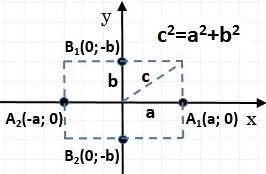
\includegraphics[width=\textwidth]{img/rettangolo.jpg}
%     \caption{Relazione tra i parametri dell' iperbole.}
    %\label{fig:ellissedalcono}
    %    \end{inaccessibleblock}
  \end{minipage}
% \end{figure}

\vspace{0.2cm}

Cerchiamo di capire la relazione tra il rettangolo appena determinato e 
l'iperbole.

% \begin{figure}[h]
  %\hspace{12pt}
  \begin{minipage}[c]{.65\textwidth}
    L'iperbole tocca il rettangolo $A_{1} A_{2} B_{1} B_{2}$ 
soltanto nei vertici reali $A_{1}$ e $A_{2}$ e si sviluppa 
illimitatamente all'interno delle due parti di piano delimitate da due 
rette, chiamate \textbf{asintoti}. Gli asintoti non sono altro che la prosecuzione 
delle diagonali del rettangolo ed hanno come coefficiente angolare $ m=\pm 
b/a$. Gli stessi asintoti forniscono una sorta di limite invalicabile e irraggiungibile
da parte dell'iperbole. Le equazioni di queste rette, 
passanti per l'origine sono $y = \pm \dfrac{b}{a} x$.
  \end{minipage}
  \hspace{.2cm}
  \begin{minipage}[c]{.3\textwidth}
    %    \begin{inaccessibleblock}[Cono a due falde tagliato da un piano
    %      che forma un'ellisse.]
    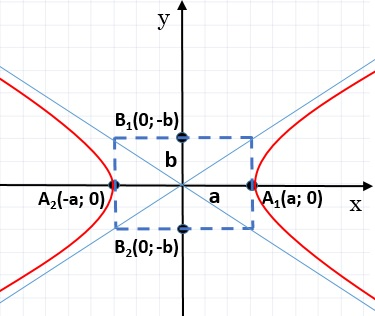
\includegraphics[width=\textwidth]{img/asintoti.jpg}
%     \caption{il rettangolo caratteristico dell'iperbole.}
    %\label{fig:ellissedalcono}
    %    \end{inaccessibleblock}
  \end{minipage}
% \end{figure}

Notiamo infine che possiamo esprimere le coordinate dei fuochi in funzione 
di a e b come: $ F_{1}(\sqrt{a^{2}+b^{2}}, 0) $, $ 
F_{2}(-\sqrt{a^{2}+b^{2}}, 0) $
\item [\textbf{Eccentricità}]: Analogamente a 
quanto visto per l'ellisse definiamo l'eccentricità di un iperbole come
rapporto tra distanza focale e lunghezza dell'asse trasverso:
\begin{equation}
e=\dfrac{\text{distanza focale}}{\text{asse trasverso}}=\dfrac{2c}{2a}=\dfrac{c}{a}=\dfrac{\sqrt{a^{2}+b^{2}}}{a}
\end{equation}
poiché dalla precedente formula $c>a$, osserviamo che $e>1$.
Per comprendere il significato geometrico dell'eccentricità e
la relazione che tale valore ha col grafico dell'iperbole, studiamo come varia 
l'eccentricità al variare di $b$ (tenendo fisso il parametro $a$), con i seguenti esempi:
\begin{figure}[htbp]
  \centering
  %    \begin{inaccessibleblock}[Cono a due falde tagliato da un piano
  %      che forma un'ellisse.]
  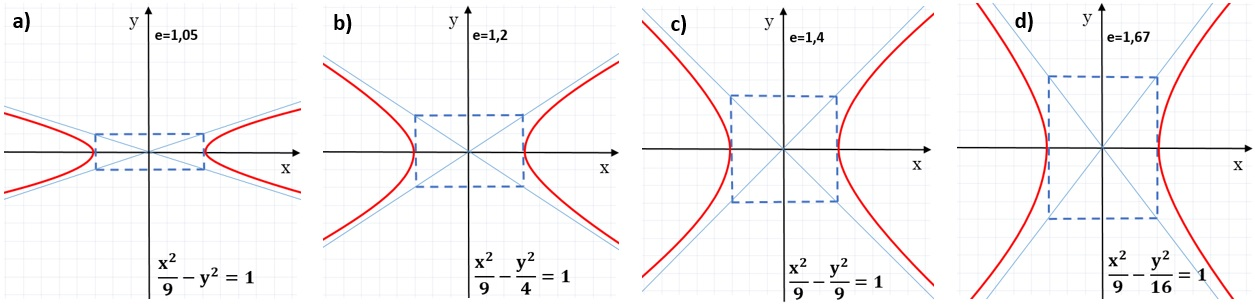
\includegraphics[width=\textwidth]{img/4iperboli.jpg}
    \caption{Eccentricità dell'iperbole al variare del 
parametro b.}%
  %\label{fig:ellissedalcono}
  %    \end{inaccessibleblock}
\end{figure}
\end{description}
In particolare, si può notare che:
\begin{itemize}
 \item $e \rightarrow 0$ (caso limite): l'iperbole tende ad appiattirsi fino a coincidere con l'asse $x$
\item $e>1$: i fuochi si allargano, determinando un'apertura dei rami dell'iperbole
\item $e \rightarrow +\infty$ (caso limite):
l'iperbole si allarga sempre più, fino a coincidere con le rette $x=\pm a$
\end{itemize}

\subsection{L'iperbole con i fuochi sull'asse Y}

Se i fuochi, al contrario di quanto visto finora, giacciono sull'asse Y e 
hanno coordinate $ F_{1} (0;~-c)$ e $ F_{2} (0;~c)$ prende forma una nuova 
tipologia di iperbole che invece di svilupparsi a sinistra e a destra 
dell'origine si sviluppa sopra e sotto di tale punto.
Con ragionamenti molto simili ai precedenti, partendo stavolta dalla relazione 
$\left|\overline{PF_{1}}-\overline{PF_{2}}\right|=2b$ riusciamo a 
determinare l'equazione canonica di questo tipo di iperbole, ovvero: 
\begin{equation}
-\dfrac{x^{2}}{a^{2}}+\dfrac{y^{2}}{b^{2}}=1
\end{equation}
Si può facilmente verificare che:
\begin{itemize} [noitemsep]
  \item l'iperbole è simmetrica rispetto all'origine e agli assi 
cartesiani ;
  \item l'asse Y è l'asse trasverso e su di esso giacciono i vertici 
reali $ B_{1} (0;~b)$ e $ B_{2} (0;~-b)$;
  \item l'asse X è l'asse non trasverso dove giacciono i vertici non 
reali $ A_{1} (a;~0)$ e $ A_{2} (-a;~0)$;
  \item le rette di equazione $y= \pm \dfrac{b}{a}  x$ sono gli asintoti dell'iperbole;
  \item l'eccentricità è definita dalla formula 
$e=\dfrac{c}{b}=\dfrac{\sqrt{b^{2}+a^{2}}}{b} $
\end{itemize}

\subsection{Condizioni per determinare l'equazione dell'iperbole}

Similmente a quanto visto per l'ellisse, poiché anche l'iperbole 
è determinata da due parametri ($a$, $b$), serviranno solo due condizioni per 
determinarne l'equazione canonica.
Le coppie di informazioni che insieme consentono di determinare un'iperbole 
sono:
\begin{itemize}[noitemsep]
\item Due punti appartenenti all'iperbole (non simmetrici rispetto 
agli assi o rispetto all'origine);
\item Punto dell'iperbole e fuoco (o vertice);
\item Fuoco e vertice;
\item Eccentricità e un fuoco (o vertice, o punto dell'iperbole);
\item Asintoto e fuoco (o vertice, o punto dell'iperbole).
\end{itemize}

\subsection{L'iperbole equilatera e la funzione omografica}
\label{subsec:iperbole_omografica}

Se le lunghezze del semiasse trasverso e non trasverso sono uguali, ovvero $a=b$, 
l'equazione dell'iperbole (con i fuochi sull'asse $x$) diventa: 
\begin{equation}
\dfrac{x^{2}}{a^{2}}-\dfrac{y^{2}}{a^{2}}=1 \qquad \longrightarrow \qquad
x^{2}-y^{2} =  a^{2} 
\end{equation}
Tale forma di iperbole, con un solo parametro, è detta 
\emph{iperbole equilatera riferita ai propri assi}. 
In questo caso gli altri elementi che caratterizzano l'iperbole diventano:

\vspace{12pt}
% \begin{figure}[h]
  %\hspace{12pt}
  \noindent\begin{minipage}[c]{.65\textwidth}
  \begin{itemize}
    \item asintoti: $y\pm=x$ (bisettrici dei quadranti);
    \item semidistanza focale: $c=a \sqrt{2} $;
    \item eccentricità: $e = \dfrac{\sqrt{a^{2}+a^{2}}}{a}=\sqrt{2} $
    \item fuochi: $ F_{1} \left(a \sqrt{2};~0\right)$ e 
                        $ F_{2}\left(-a \sqrt{2};~0\right)$
    \item vertici reali: $ A_{1}(a;~0)$ e $A_{2}(-a;~0)$
  \end{itemize}    
  \end{minipage}
  \hfill
  \begin{minipage}[c]{.3\textwidth}
    %    \begin{inaccessibleblock}[Cono a due falde tagliato da un piano
    %      che forma un'ellisse.]
    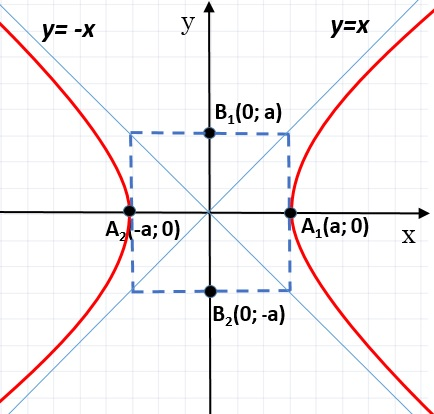
\includegraphics[height=4cm, width=4cm,]{img/equilatera.jpg}
%     \caption{L'iperbole equilatera.}
    %\label{fig:ellissedalcono}
    %    \end{inaccessibleblock}
  \end{minipage}
% \end{figure}

\vspace{12pt}
Da notare che il rettangolo, costruito con i vertici, in questo caso diventa un quadrato di lato pari a $2a$.
Nel caso simmetrico, con i fuochi sull'asse Y, l'equazione diventa:
$ x^{2} - y^{2} =- a^{2} $, con i fuochi 
$ F_{1} \left(0; a \sqrt{2}\right)$, $ F_{2} \left(0;~-a \sqrt{2}\right)$ 
e vertici reali $ B_{1} (0; a)$,$ B_{2} (0; -a)$.

\vspace{7pt}

Ruotando di $45\grado$ l'iperbole equilatera riferita ai propri 
assi otteniamo una nuova iperbole che ha come asintoti gli assi cartesiani 
e come assi di simmetria le bisettrici dei quadranti.
Chiamiamo questo tipo 
di iperbole \emph{iperbole equilatera riferita ai propri asintoti}.

Si può dimostrare che l'equazione di tale iperbole si può scrivere nella 
forma: 
\begin{equation}
x y=k \hspace{1cm} con \hspace{0.2cm}k \neq 0
\end{equation}
In figura \ref{fig:iperboleequilatera} è possibile vedere il grafico di tale iperbole, nei casi $k>0$ e $k<0$.
\begin{figure}[!h]
  \centering
  %    \begin{inaccessibleblock}[Cono a due falde tagliato da un piano
  %      che forma un'ellisse.]
  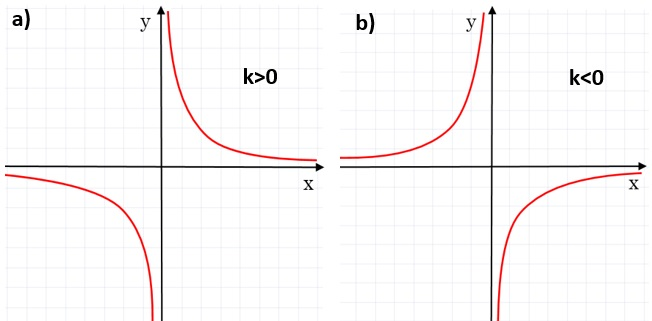
\includegraphics[height=6cm, width=10.5cm]{img/equilatera2.jpg}
  \caption{Iperbole equilatera con k>0 e k<0.}
  \label{fig:iperboleequilatera}
  %    \end{inaccessibleblock}
\end{figure}

\vspace{7pt}

Notiamo che l'equazione $xy=k$ non è altro che l'espressione della 
proporzionalità inversa tra due grandezze che mantengono costante il loro 
prodotto, dove $k$ è la costante di proporzionalità. Soffermiamoci sulla 
figura \ref{fig:iperboleequilatera}: i vertici di quest'iperbole, utili per disegnarla, sono dati 
dall'intersezione dell'iperbole con la bisettrice del primo e terzo 
quadrante (oppure secondo e quarto, a seconda del segno di $k$). Intersecando l'iperbole $xy=k$ (con $k>0$)
e la bisettrice $y=x$ otteniamo: $A_{1} \punto{\sqrt{k}}{\sqrt{k}}$ e 
$A_{2} \punto{- \sqrt{k}}{-\sqrt{k}}$. Nel caso di $k<0$ cambiano solamente i segni (e si mette $|k|$ all'interno delle radici), che in ogni caso
si possono dedurre in modo semplice dal grafico, ragionando sui quadranti. I fuochi hanno invece coordinate
$F_1 \punto{\sqrt{2k}}{\sqrt{2k}}$ e $F_2 \punto{-\sqrt{2k}}{-\sqrt{2k}}$, con analogo ragionamento sui segni
nel caso $k<0$

\vspace{12pt}

\noindent\begin{minipage}{.6\textwidth}
L'ultima tipologia di iperbole, ampiamente utilizzata in matematica,
è la cosiddetta \emph{funzione omografica}. Si tratta semplicemente di
una traslazione di un'iperbole equilatera riferita ai propri asintoti (ovvero $xy=k$).
L'equazione che ne deriva ha la seguente forma:
\begin{equation}
y= \dfrac{ax+b}{cx+d}
\end{equation}

con $a,b,c,d\in \R$, $c \neq 0$ e $ ad-bc \neq 0$

\vspace{6pt}
Il centro e gli asintoti di quest'iperbole sono:
\[C \punto{-\dfrac{d}{c}}{\dfrac{a}{c}} \qquad y= \dfrac{a}{c} \quad; \quad  x=-\dfrac{d}{c}\]
\end{minipage}
\hfill
\begin{minipage}{.35\textwidth}
% \begin{figure}[!htbp]
  \centering
  %    \begin{inaccessibleblock}[Cono a due falde tagliato da un piano
  %      che forma un'ellisse.]
  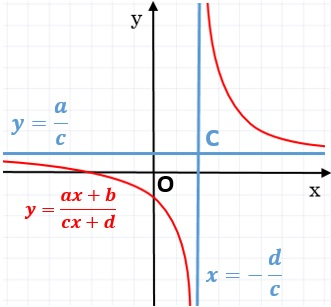
\includegraphics[height=5cm, width=5cm]{img/omografica.jpg}
%   \caption{Funzione omografica.}%
  %\label{fig:ellissedalcono}
  %    \end{inaccessibleblock}
% \end{figure}
\end{minipage}

\vspace{15pt}
Le due condizioni precedentemente poste nell'equazione della funzione omografica
sono molto importanti, infatti:

\begin{itemize} [noitemsep]
  \item se $c= 0$ otteniamo $y= \dfrac{ax+b}{d} $ cioè $y= 
\dfrac{ax}{d} + \dfrac{b}{d} $, che rappresenta una semplice retta; \\[3pt]
  \item se $ad-bc=0$, ovvero $ \dfrac{d}{c} = \dfrac{b}{a} $, supponendo $x\neq-d/c$, si ha: 
\[y=\dfrac{ax+b}{cx+d}=  \dfrac{a\left(x+ \frac{b}{a} \right)}{c\left(x+ 
\frac{d}{c} \right)} = \dfrac{a \cancel{\tonda{x+ \frac{b}{a}}}}{c\cancel{\tonda{x+ 
\frac{b}{a} }}} = 
\dfrac{a}{c} \] e quindi otteniamo una retta parallela all'asse $x$, di equazione $y=a/c$, 
definita per tutti valori di $x$, tranne $x=-d/c$.  
\end{itemize}

Come si disegna una funzione omografica? Inizialmente si determinano il centro e gli asintoti,
usando le formule descritte in precendenza. Quindi, per ricavare i vertici dell'iperbole è
sufficiente trovare l'intersezione di quest'ultima con la parallela alla bisettrice del
primo/terzo quadrante passante per il centro dell'iperbole, ovvero $y-y_C = \pm (x-x_C)$.

\begin{esempio}
~

% \begin{figure}[h]
  %\hspace{12pt}
  \begin{minipage}[c]{.6\textwidth}
    \emph{Data l'iperbole equilatera $ x^{2} - y^{2} =6$, determina 
vertici, fuochi e corrispondente grafico.}\\[7pt]
    Poiché $a= \sqrt{6} $, i vertici reali sono dati dai punti $ A_{1} 
\punto{\sqrt{6}}{0}$ e $ A_{2} 
\punto{-\sqrt{6}}{0}$. Il parametro $c$ si può calcolare con:
\[c=\sqrt{6}  \sqrt{2} = \sqrt{12} =2 \sqrt{3}\] Grazie a $c$ 
calcoliamo i fuochi $ F = \punto{\pm 2\sqrt{3}}{0}$. Il grafico
corrispondente è disegnato a lato.
  \end{minipage}
  \hspace{.2cm}
  \begin{minipage}[c]{.35\textwidth}
    %    \begin{inaccessibleblock}[Cono a due falde tagliato da un piano
    %      che forma un'ellisse.]
    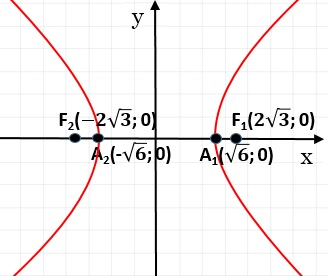
\includegraphics[width=\textwidth]{img/equilatera1.jpg}
    %\caption{Generazione di un'ellisse da un cono a due falde}
    %\label{fig:ellissedalcono}
    %    \end{inaccessibleblock}
  \end{minipage}
% \end{figure}
\end{esempio}

\newpage %--------------------------------------------------

\begin{esempio}
~

% \begin{figure}[h]
  %\hspace{12pt}
  \begin{minipage}[c]{.6\textwidth}
    \emph{Data l'iperbole equilatera $xy=8$, determina vertici, fuochi 
e corrispondente grafico.}

\vspace{7pt}

Si tratta di un'iperbole equilatera riferita ai propri 
asintoti e, poiché $k> 0$, si trova nel primo e terzo quadrante. I vertici 
sono: $ A_{1} \punto{2\sqrt{2}}{2\sqrt{2}}$ e $ A_{2} 
\punto{-2\sqrt{2}}{-2\sqrt{2}}$. I fuochi avranno quindi coordinate 
$ F_{1} \punto{4}{4}$ e $ F_{2} \punto{-4}{-4}$
  \end{minipage}
  \hspace{.2cm}
  \begin{minipage}[c]{.35\textwidth}
    %    \begin{inaccessibleblock}[Cono a due falde tagliato da un piano
    %      che forma un'ellisse.]
    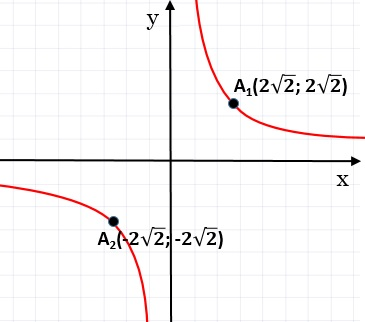
\includegraphics[width=\textwidth]{img/equilatera2a.jpg}
    %\caption{Generazione di un'ellisse da un cono a due falde}
    %\label{fig:ellissedalcono}
    %    \end{inaccessibleblock}
  \end{minipage}
% \end{figure}
\end{esempio}

\begin{esempio} \emph{Data la funzione omografica $y= \dfrac{x-3}{x+2}$, 
dopo aver verificato che è un'iperbole , determinane gli 
asintoti e il centro di simmetria. Completa l'esercizio disegnando il grafico della funzione.}\\[7pt]
Per verificare se si tratta di un iperbole, è sufficiente vedere che 
$c=1\neq 0$ e che $ad-bc=5\neq 0$. 
Possiamo ora determinare gli asintoti: quello verticale è 
$x=- \dfrac{d}{c} =-2$ e quello orizzontale è $y= \dfrac{a}{c} =1$; 
il centro di simmetria è $C(-2; ~1)$.

\noindent \begin{minipage}[c]{.65\textwidth}
Per disegnare la funzione, una volta inseriti gli asintoti, è possibile andare
a calcolare le intersezioni dell'iperbole con l'asse $x$ e l'asse $y$, in modo
da avere qualche punto di riferimento per il grafico (e i corrispondenti punti simmetrici
rispetto al centro dell'iperbole). Calcolando, si trova: $ P_{1}  \left(0;~ - \dfrac{3}{2} \right)$ e $ P_{2} =(3;~0)$.
  \end{minipage}
  \hspace{0.5cm}
  \begin{minipage}[c]{.3\textwidth}
    %    \begin{inaccessibleblock}[Cono a due falde tagliato da un piano
    %      che forma un'ellisse.]
    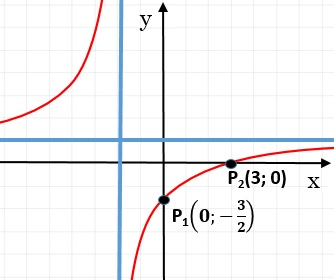
\includegraphics[width=\textwidth]{img/equilatera2b.jpg}
    %\caption{Generazione di un'ellisse da un cono a due falde}
    %\label{fig:ellissedalcono}
    %    \end{inaccessibleblock}
  \end{minipage}
% \end{figure}
\end{esempio}


  


